\section{Lernfeld 6 - Programmieren}

%%% Anfang: tl;dr
\subsection{tl;dr - Zusammenfassung der Zusammenfassung}
%%% Ende: tl;dr
%%%%%%%%%%%%%%%%%%%%%%%%%%%%%%%%%%%%%%%%%%%%%%%%%%%%%%%%%%%%%%%%%%%%%%%%%%%%%%%%

%%% Anfang: HTML / PHP
\subsection{Einführung in HTML und PHP}

HTML ist, wie der Name -- HyperText Markup Language -- schon sagt, eine Beschreibungsssprache. Im Gegensatz zu Word sieht das interpretierte Ergebnis eines HTML-Dokuments nicht so aus, wie sie geschrieben wurde. HTML ist also eher mit \LaTeX zu vergleich.

In den folgenden Abschnitten werden zunächst die wichtigsten Tags beschrieben, um HTML-Dokumente zu strukturieren. Anschließend werden die Möglichkeiten von HTML anhand von Aufgaben und deren Lösungen dargestellt.

%%% Anfang: LS01 > Kurzreferenz
\subsubsection{HTML5: Kurzreferenz}
In diesem Abschnitt werden die wichtigsten Tags beschrieben, um ein HTML-Dokument zu strukturieren. Alle erwähnten Dateien befinden sich unter \texttt{code/lf06prog-code}.\newline

{\bf Überschriften}.\ \ Ähnlich wie in TeX können Überschriften in mehreren Ebenen beschrieben werden. Wo TeX bloß drei Ebenen vorsieht (\verb+\section, \subsection} und \subsubsection+), sind durch HTML prinzipiell keine Grenzen gesetzt. Überschriften werden in HTML durch die Tags \texttt{<hX>} und \texttt{</hX>} beschrieben. Dabei steht X für die jeweilige Hierarchie. Abhängig von X wird die Größe der Überschrift gesetzt. Die Datei \texttt{lf06prog-headlines.html} macht das Beschriebene anschaulich.\newline

{\bf Absätze}.\ \ Möchte man einen Textblock als zusammengehörigen Absatz definieren, setzt man dafür die Tags \texttt{<p>} und \texttt{</p>}. Harte Zeilenumbrüche werden durch das einzelne Tag \texttt{<br />} beschrieben. Weil zwischen den Tags \texttt{<br> <br/>} eh nichts steht, wurde dieses vereinfacht. Daher ist auf das Leerzeichen in \texttt{<br />} zu achten.\newline

{\bf Hervorhebungen}.\\
\begin{tabular}{lll}
\texttt{<b> </b>} & {\bf fett} (physikalisch $\widehat{=}$ Stilelement) & \\
\texttt{<strong> </strong>} & {\bf fett} (logisch $\widehat{=}$ wichtig) & \\
\texttt{<i> </i>} & {\it kursiv} & \\
\texttt{<em> </em>} & betont; meist {\it kursiv} & \\
\texttt{<sup> </sup>} & $^{hochgestellt}$ & \\
\texttt{<sub> </sub>} & $_{tiefgestellt}$ & \\
\texttt{<u> </u>} & \sout{durchgestrichen} & \\
\end{tabular}\newline

{\bf Listen}.\ \ Mit den Tags \texttt{<ul> </ul>} und \texttt{<ol> </ol>} lassen sich Listen definieren. \texttt{<li> </li>} definieren jeweils die Listenelemente, wobei den Listenelementen bei \texttt{<ul>} ein Punkt vorangestellt wird und bei \texttt{<ol>} die Listenelemente durchnummeriert werden. Siehe dazu auch \texttt{lf06prog-listen.html} und \url{http://wiki.selfhtml.org/wiki/HTML/Textstrukturierung/Listen}.\newline

{\bf Umlaute}.\ \ HTML kann Umlaute nicht ohne weiteres darstellen. Daher müssen Umlaute durch die folgenden Befehle definiert werden:\\
\begin{tabular}{ll}
ä & \&auml;\\
Ä & \&Auml;\\
ö & \&ouml;\\
Ö & \&Ouml;\\
ü & \&uuml;\\
Ü & \&Uuml;\\
ß & \&szlig;\\
\euro & \&euro;\\
\end{tabular}\newline

{\bf Tabellen}.\ \ Besondere Bedeutung in HTML haben Tabellen. Mit diesen lässt sich der Aufbau einer Seite gestalten. Statt den Aufbau von Tabellen umständlich zu beschreiben, verweise ich auf die Datei \texttt{lf06prog-listen.html}. Diese sollte sich sowohl als Quellcode als auch im Browser angesehen werden.\newline

{\bf Links}. . .\ \ sind einer der großen Fortschritte, die das Internet erst zu dem machen, was es ist.
\begin{tabular}{lll}
Interner Link & \verb+<a href="interner-link.html">Beschreibung</a>+ &\\
Externer Link & \verb+<a href=\"https://externer-link.html\">Beschreibung</a>+ &\\
Link auf Bild & \verb+<a href=\"lokales-bild.jpg\">Bild</a>+ &\\
Link auf PDF & \verb+<a href=\"lokales-pdf.pdf\">Beschreibung</a>+ &\\
Mail als Link & \verb+<a href=\"mailto:email@email.email\">Schreib mich an!</a>+ &\\
Sprungmarke & \verb+<a href="\#anker">Spring zu Anker</a>+ &\\
& benötigt: \verb+<a name=\"anker\">Anker</a>+ &\\
\end{tabular}\newline

{\bf Grafiken}.\\
\verb+<img src="bild.jpg" width="" height="" border="0" alt="" title="" />+\\
\begin{tabular}{ll}
src & Wo die Datei liegt\\
width & Wie breit das Bild dargestellt werden soll\\
height & Wie hoch das Bild dargestellt werden soll\\
border & Rahmen?\\
alt & Beschreibung des Bildes\\
title & Titel des Bildes\\
\end{tabular}\newline

{\bf Kommentare}. . .\ \ lassen sich in HTML-Dokumenten einfügen, indem sie zwischen \verb+<!-- -->+ geschrieben werden.

%%% Anfang: HTML / PHP > Aufgaben
\subsubsection{Aufgaben: HTML und PHP}



%%% Ende: HTML / PHP
%%%%%%%%%%%%%%%%%%%%%%%%%%%%%%%%%%%%%%%%%%%%%%%%%%%%%%%%%%%%%%%%%%%%%%%%%%%%%%%%

%%% Anfang: Struktogramm
\subsection{Struktogramm und Ablaufplan}


%%% Ende: Struktogramm
%%%%%%%%%%%%%%%%%%%%%%%%%%%%%%%%%%%%%%%%%%%%%%%%%%%%%%%%%%%%%%%%%%%%%%%%%%%%%%%%

%%% Anfang: Verzweigung
\subsection{Einführung in Verzweigungen}

%%% Anfang: Verzweigung > Schleifen
\subsubsection{Schleifen}

\paragraph{Kopfgesteuerte Schleife}~\\

\paragraph{Fußgesteuerte Schleife}~\\

\subsubsection{IF}

\subsubsection{FOR - Zählschleife}

\includegraphics[scale=0.4]{pictures/lf06prog-pic/lf06prog-for-pap.png}
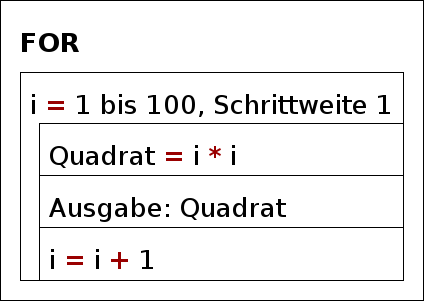
\includegraphics[scale=0.4]{pictures/lf06prog-pic/lf06prog-for-struct.png}

\subsubsection{WHILE}

% While: Fuss
\includegraphics[scale=0.4]{pictures/lf06prog-pic/lf06prog-while-fuss.png}
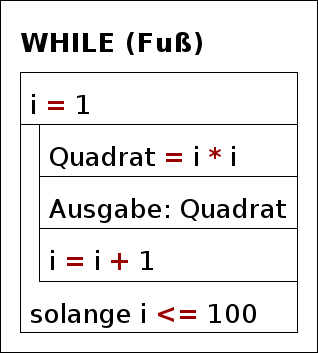
\includegraphics[scale=0.4]{pictures/lf06prog-pic/lf06prog-while-fuss-struct.png}

% While: Kopf
\includegraphics[scale=0.4]{pictures/lf06prog-pic/lf06prog-while-kopf.png}
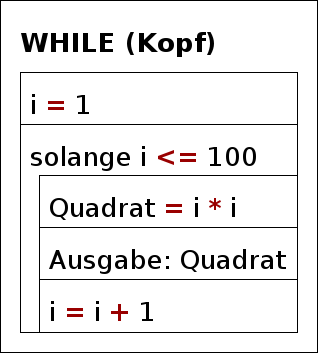
\includegraphics[scale=0.4]{pictures/lf06prog-pic/lf06prog-while-kopf-struct.png}

%%% Anfang: Verzweigung > Switch
\subsubsection{Switch-Case}
\begin{tabular}{l|l|l}

\end{tabular}
\lstinputlisting
	[caption={Ein Beispiel für Switch-Case-Anweisungen}
	\label{lst:Switch-Case},captionpos=b,language=PHP]
	{code/lf06prog-code/lf06prog-switch.case.php}

\subsubsection{Arrays}

\paragraph{Indexorientierte Arrays}~\\

\paragraph{Assoziative Arrays}~\\

%%% Ende: Verzweigung
%%%%%%%%%%%%%%%%%%%%%%%%%%%%%%%%%%%%%%%%%%%%%%%%%%%%%%%%%%%%%%%%%%%%%%%%%%%%%%%%